\section{Bunching and the limits of band-calibrated synthetic data}
\label{sec:bunching}

This section applies the polynomial counterfactual-density estimator of
\citet{chettyetal2011} and \citet{klevenwaseem2013}---as applied to UK VAT
data by \citet{liuetal2021}---to the synthetic firm population. Its finding is
about the data, not about firm behaviour: every sub-band feature of a
band-calibrated synthetic population is exactly what its targets put there,
and this section demonstrates the point in three directions. The 2023--24
population's near-threshold density is calibrated to the OBR's published
\pounds1{,}000-band profile (Section~\ref{sec:data}), and the estimator reads
that profile back as excess mass---target inheritance, not behaviour. A
placebo that regenerates the population \emph{without} those targets returns
zero. And the 2024--25 vintage, for which no fine bands are published,
produces a very large \emph{spurious} excess-mass signal sitting exactly on an
HMRC calibration-band edge. Together with a power (recovery) test, these
results establish the section's transparency claim: band-calibrated synthetic
data support no bunching inference in either direction, and any sub-band
feature of such data should be traced to its calibration targets before it is
read as economics. The behavioural evidence on UK VAT bunching remains the
administrative estimate of \citet{liuetal2021}.

The section also documents a correction. An earlier draft of this paper
reported an excess mass of $8{,}712$ firms at
\pounds85{,}000 that appeared to ``reproduce'' the density step documented in
administrative data. That excess mass was an artifact of a liability
mis-scaling in the generator (net liability set to value added itself rather
than the standard rate applied to value added, inflating per-firm liabilities
roughly fivefold; Section~\ref{sec:data}, footnote), which distorted how the
weight optimiser distributed mass near the threshold. Correcting the scaling
removed the step entirely; the near-threshold profile is now supplied by the
OBR targets instead, as published data rather than an optimiser
side-effect.\footnote{The defect and its diagnosis are recorded
in the replication repository (issue \#15); the near-threshold targets are
issue \#23. Aggregate calibration scores
barely moved under either change---the optimiser hit the band totals every
time---which is itself part of the lesson: aggregate fit does not discipline
sub-band shape.} A plausible-looking, literature-adjacent bunching statistic
was manufactured by an accounting bug in the data layer and survived until the
liability accounting was audited. I report this openly because it is the
sharpest available demonstration of the section's thesis.

\subsection{Methodology}

Following \citet{liuetal2021}, I group firms into fine turnover bins of
\pounds1{,}000 and estimate a counterfactual density---the distribution that would
obtain absent the registration notch---by polynomial regression on bin counts,
excluding a manipulation window around the threshold $y^{*}$:
\[
  c_j \;=\; \sum_{l=0}^{q} \beta_l \, (y_j)^{l}
  \;+\; \sum_{i \in [y^{*}_{-},\, y^{*}_{+}]} \gamma_i \, \mathbb{1}\{j = i\}
  \;+\; \varepsilon_j ,
\]
where $c_j$ is the number of firms in bin $j$, $y_j$ is the distance of bin $j$
from the threshold, $q$ is the polynomial order, and $[y^{*}_{-},\,y^{*}_{+}]$
is the excluded window. The fitted polynomial is then projected into the
excluded region to recover the counterfactual density $g(y)$, with a
mass-conservation restriction that locates the upper edge of the manipulation
window endogenously (excess mass below the threshold must equal missing mass
above it; Appendix~\ref{app:inference}). Excess bunching is the integrated
difference between the observed and counterfactual densities just below the
threshold,
\[
  B(y^{*}) \;=\; \int_{y^{*}-\Delta y^{*}}^{y^{*}} g(y)\,\mathrm{d}y
  \;\approx\; g(y^{*})\,\Delta y^{*},
\]
the approximation holding when $g$ is locally smooth. The bunching ratio
$b(y^{*}) = B(y^{*})/g(y^{*}) \approx \Delta y^{*}/y^{*}$ is the width of the
bunching region expressed as a fraction of the threshold---a normalised
\emph{ratio}, not an elasticity. The estimator delivers the raw geometry of any
density step at the threshold; whether that step reflects firm behaviour is a
separate question. The estimator reports geometry only ($b$, excess mass $E$,
and the mass-conservation objects): no elasticity is computed from it, both
because the identification critique of bunching designs applies
\citep{blomquistetal2021,bertanhaetal2023} and because on these data there is
no behavioural mass to convert.

\subsection{Results: a target-inherited signal at \pounds85{,}000, a spurious one at \pounds90{,}000}

Applied to the 2023--24 population at the \pounds85{,}000 threshold, the
estimator returns an excess mass of $E = 14{,}663$ weighted firms (bootstrap
SE $526$) and a bunching ratio $b = 0.109$ (SE $0.004$): it reads back the
bunching profile that the OBR \pounds1{,}000-band targets place in the file
(Section~\ref{sec:data}). This is target inheritance, not behaviour---the
generator contains no firm location-choice---and the placebo below proves it
by deletion. On the \citet{liuetal2021} normalisation the target-inherited
excess is $b_{\mathrm{LLAT}} = 2.86$, roughly twice their administrative
$1.361$; the two are not comparable estimates of the same object, since LLAT's
sample ends in 2014--15 while the OBR profile embeds the far deeper bunching
of the frozen-threshold era (their bunching counts nearly double between
2017--18 and 2025--26).

Applied to the 2024--25 population at the \pounds90{,}000 threshold, the same
estimator returns an enormous apparent signal: excess mass of about
$195{,}900$ weighted firms, with the manipulation-window edge pinned at the
search bound---roughly fifteen times the administrative excess-bunching ratio
of \citet{liuetal2021} on the like-for-like normalisation. No reading of the
administrative literature supports a response of this size; it is a
calibration artifact sitting exactly on the \pounds90{,}000 HMRC band edge for
that vintage, where the \pounds1--\pounds90{,}000 and
\pounds90{,}000--\pounds150{,}000 band targets meet. The pair of results is
the section's central exhibit (Figure~\ref{fig:bunch85}): where fine targets
exist, the estimator recovers exactly the shape they encode; where they do
not, it reads a band-scale discontinuity as a bunching signal an order of
magnitude beyond anything behavioural---and both readings are properties of
the targets, not of firms. Specification sensitivity separates the two cases:
the target-inherited excess at \pounds85{,}000 varies with the polynomial
degree and window (roughly $8{,}000$--$15{,}000$ in the interior cells), as a
local data feature should, while the \pounds90{,}000 artifact is
$195{,}000$--$212{,}000$ in \emph{every} cell of the grid
(Appendix~\ref{app:inference}).

\begin{figure}[htbp]
\centering
\subfigure[2023--24 population, \pounds85{,}000: target-inherited profile]{
    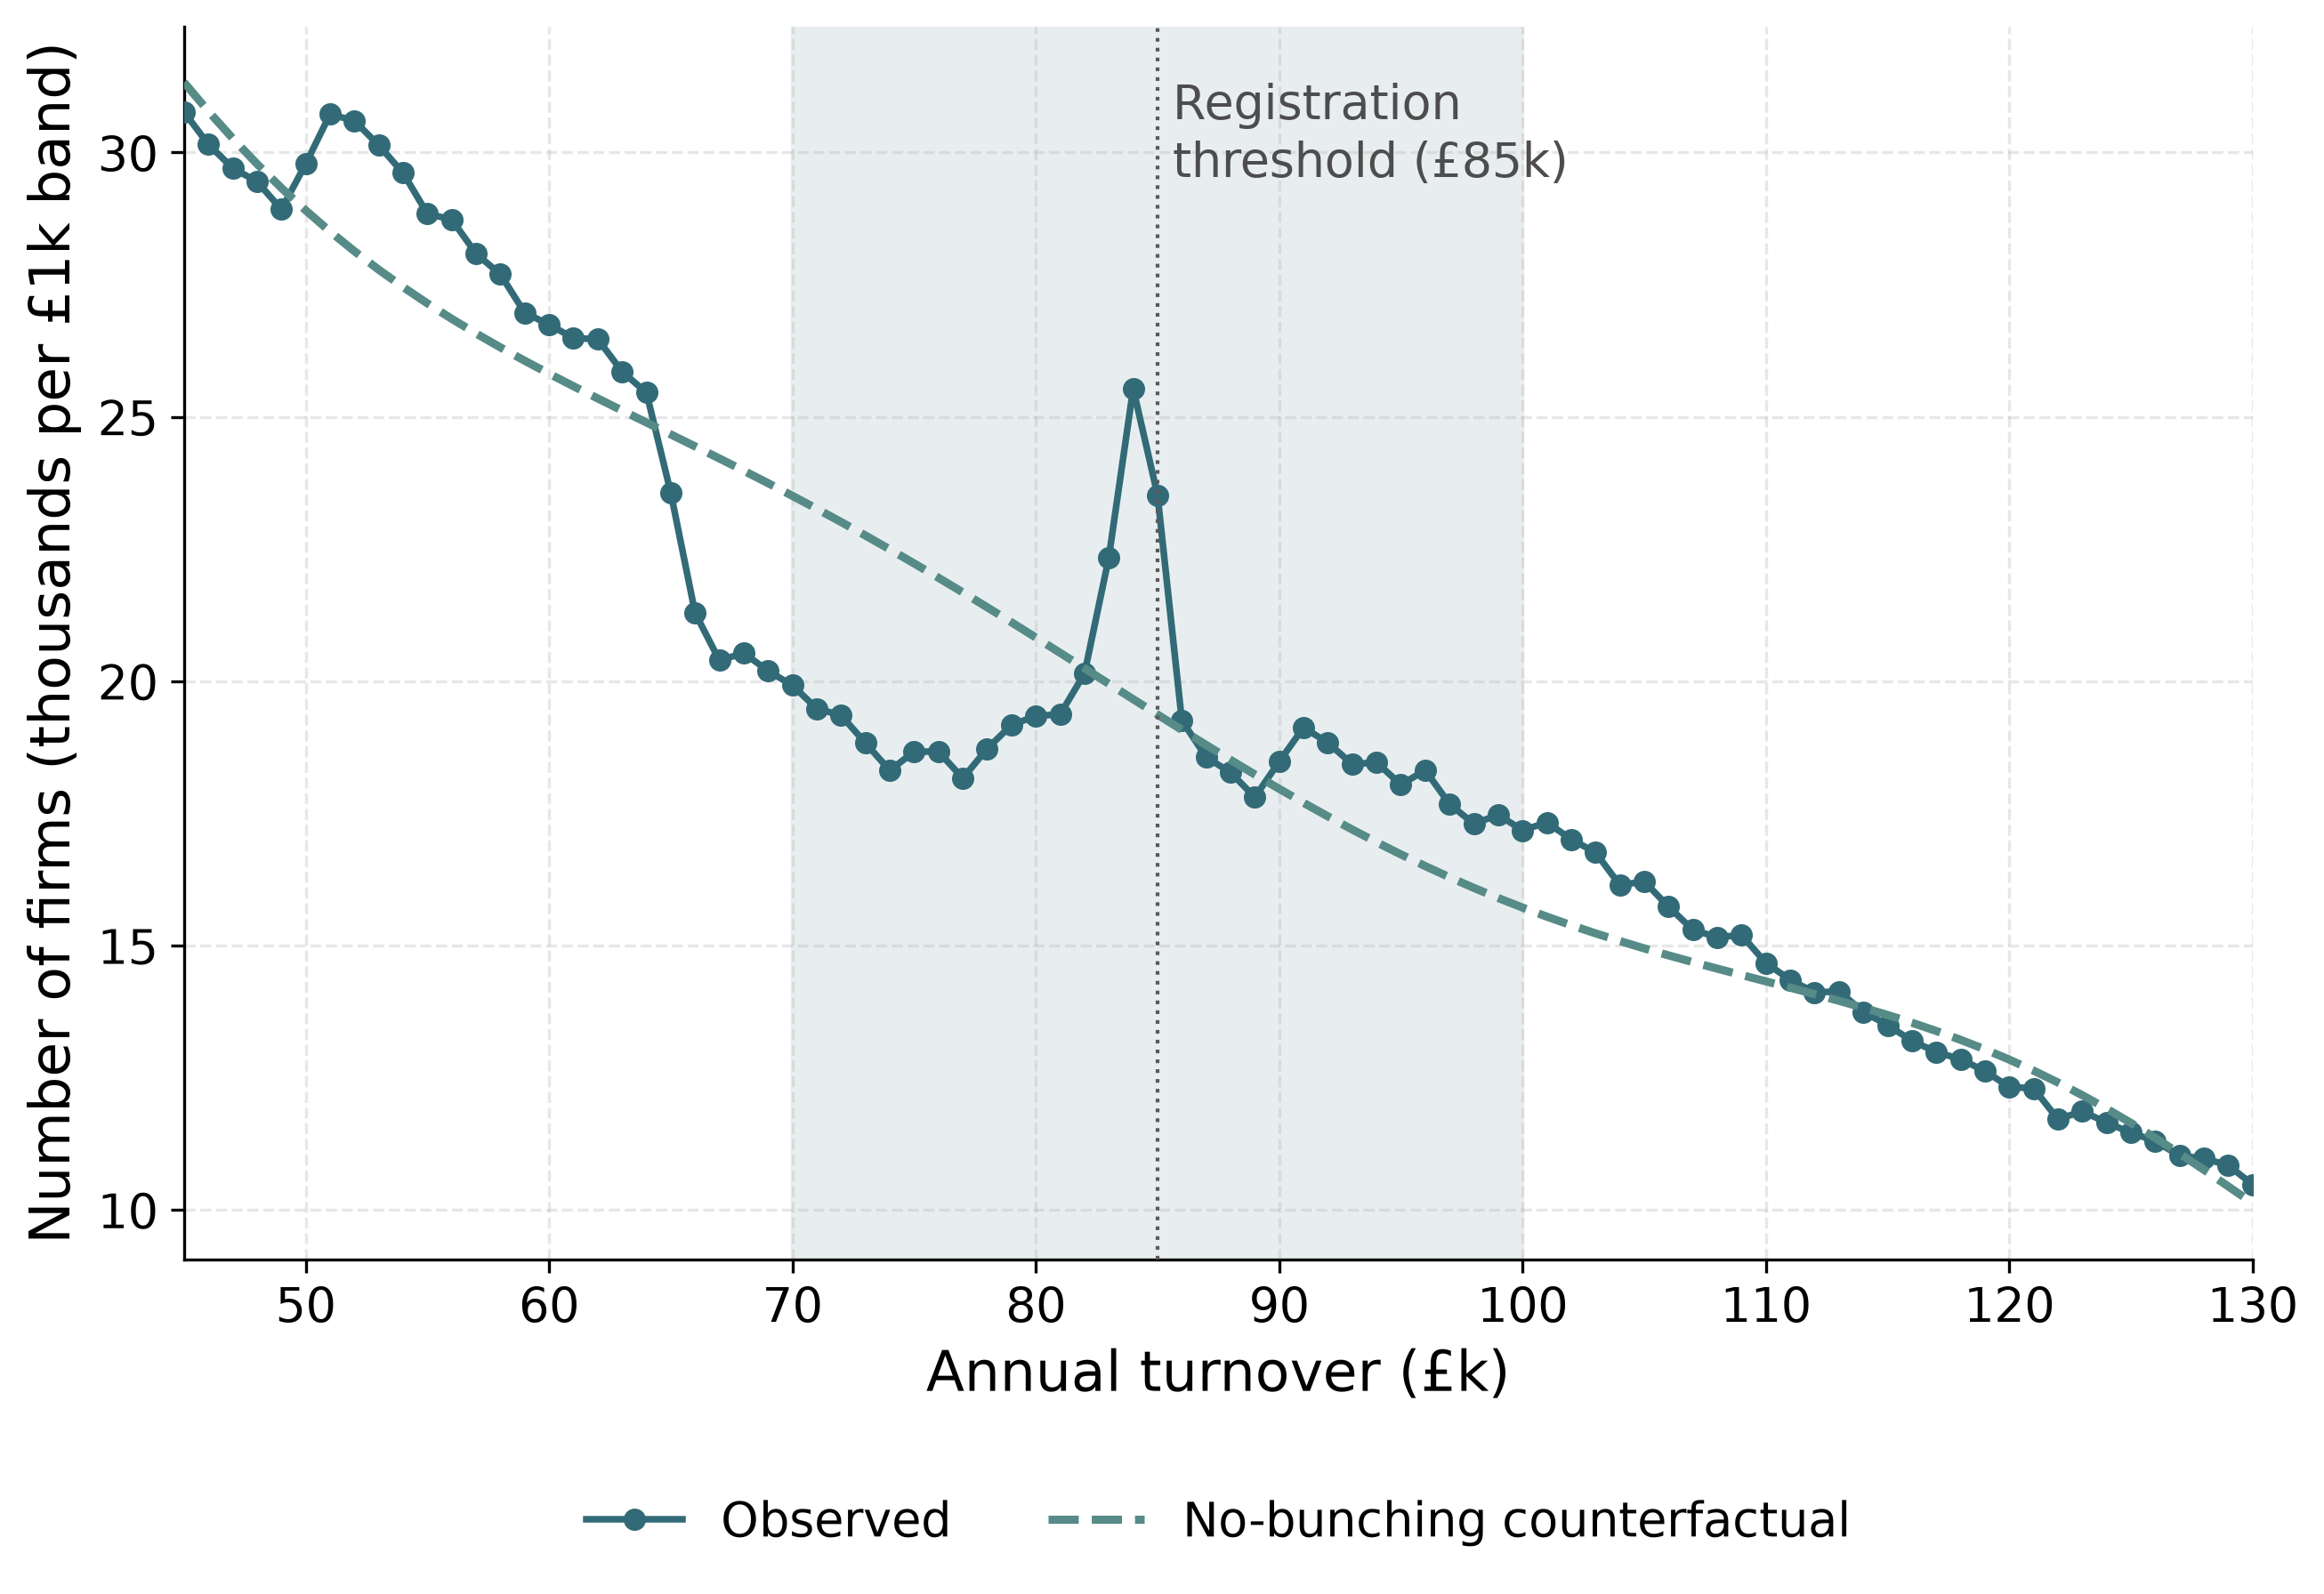
\includegraphics[width=0.48\textwidth]{figures/bunching_analysis_85k.png}
}
\hfill
\subfigure[2024--25 population, \pounds90{,}000 threshold: spurious excess mass]{
    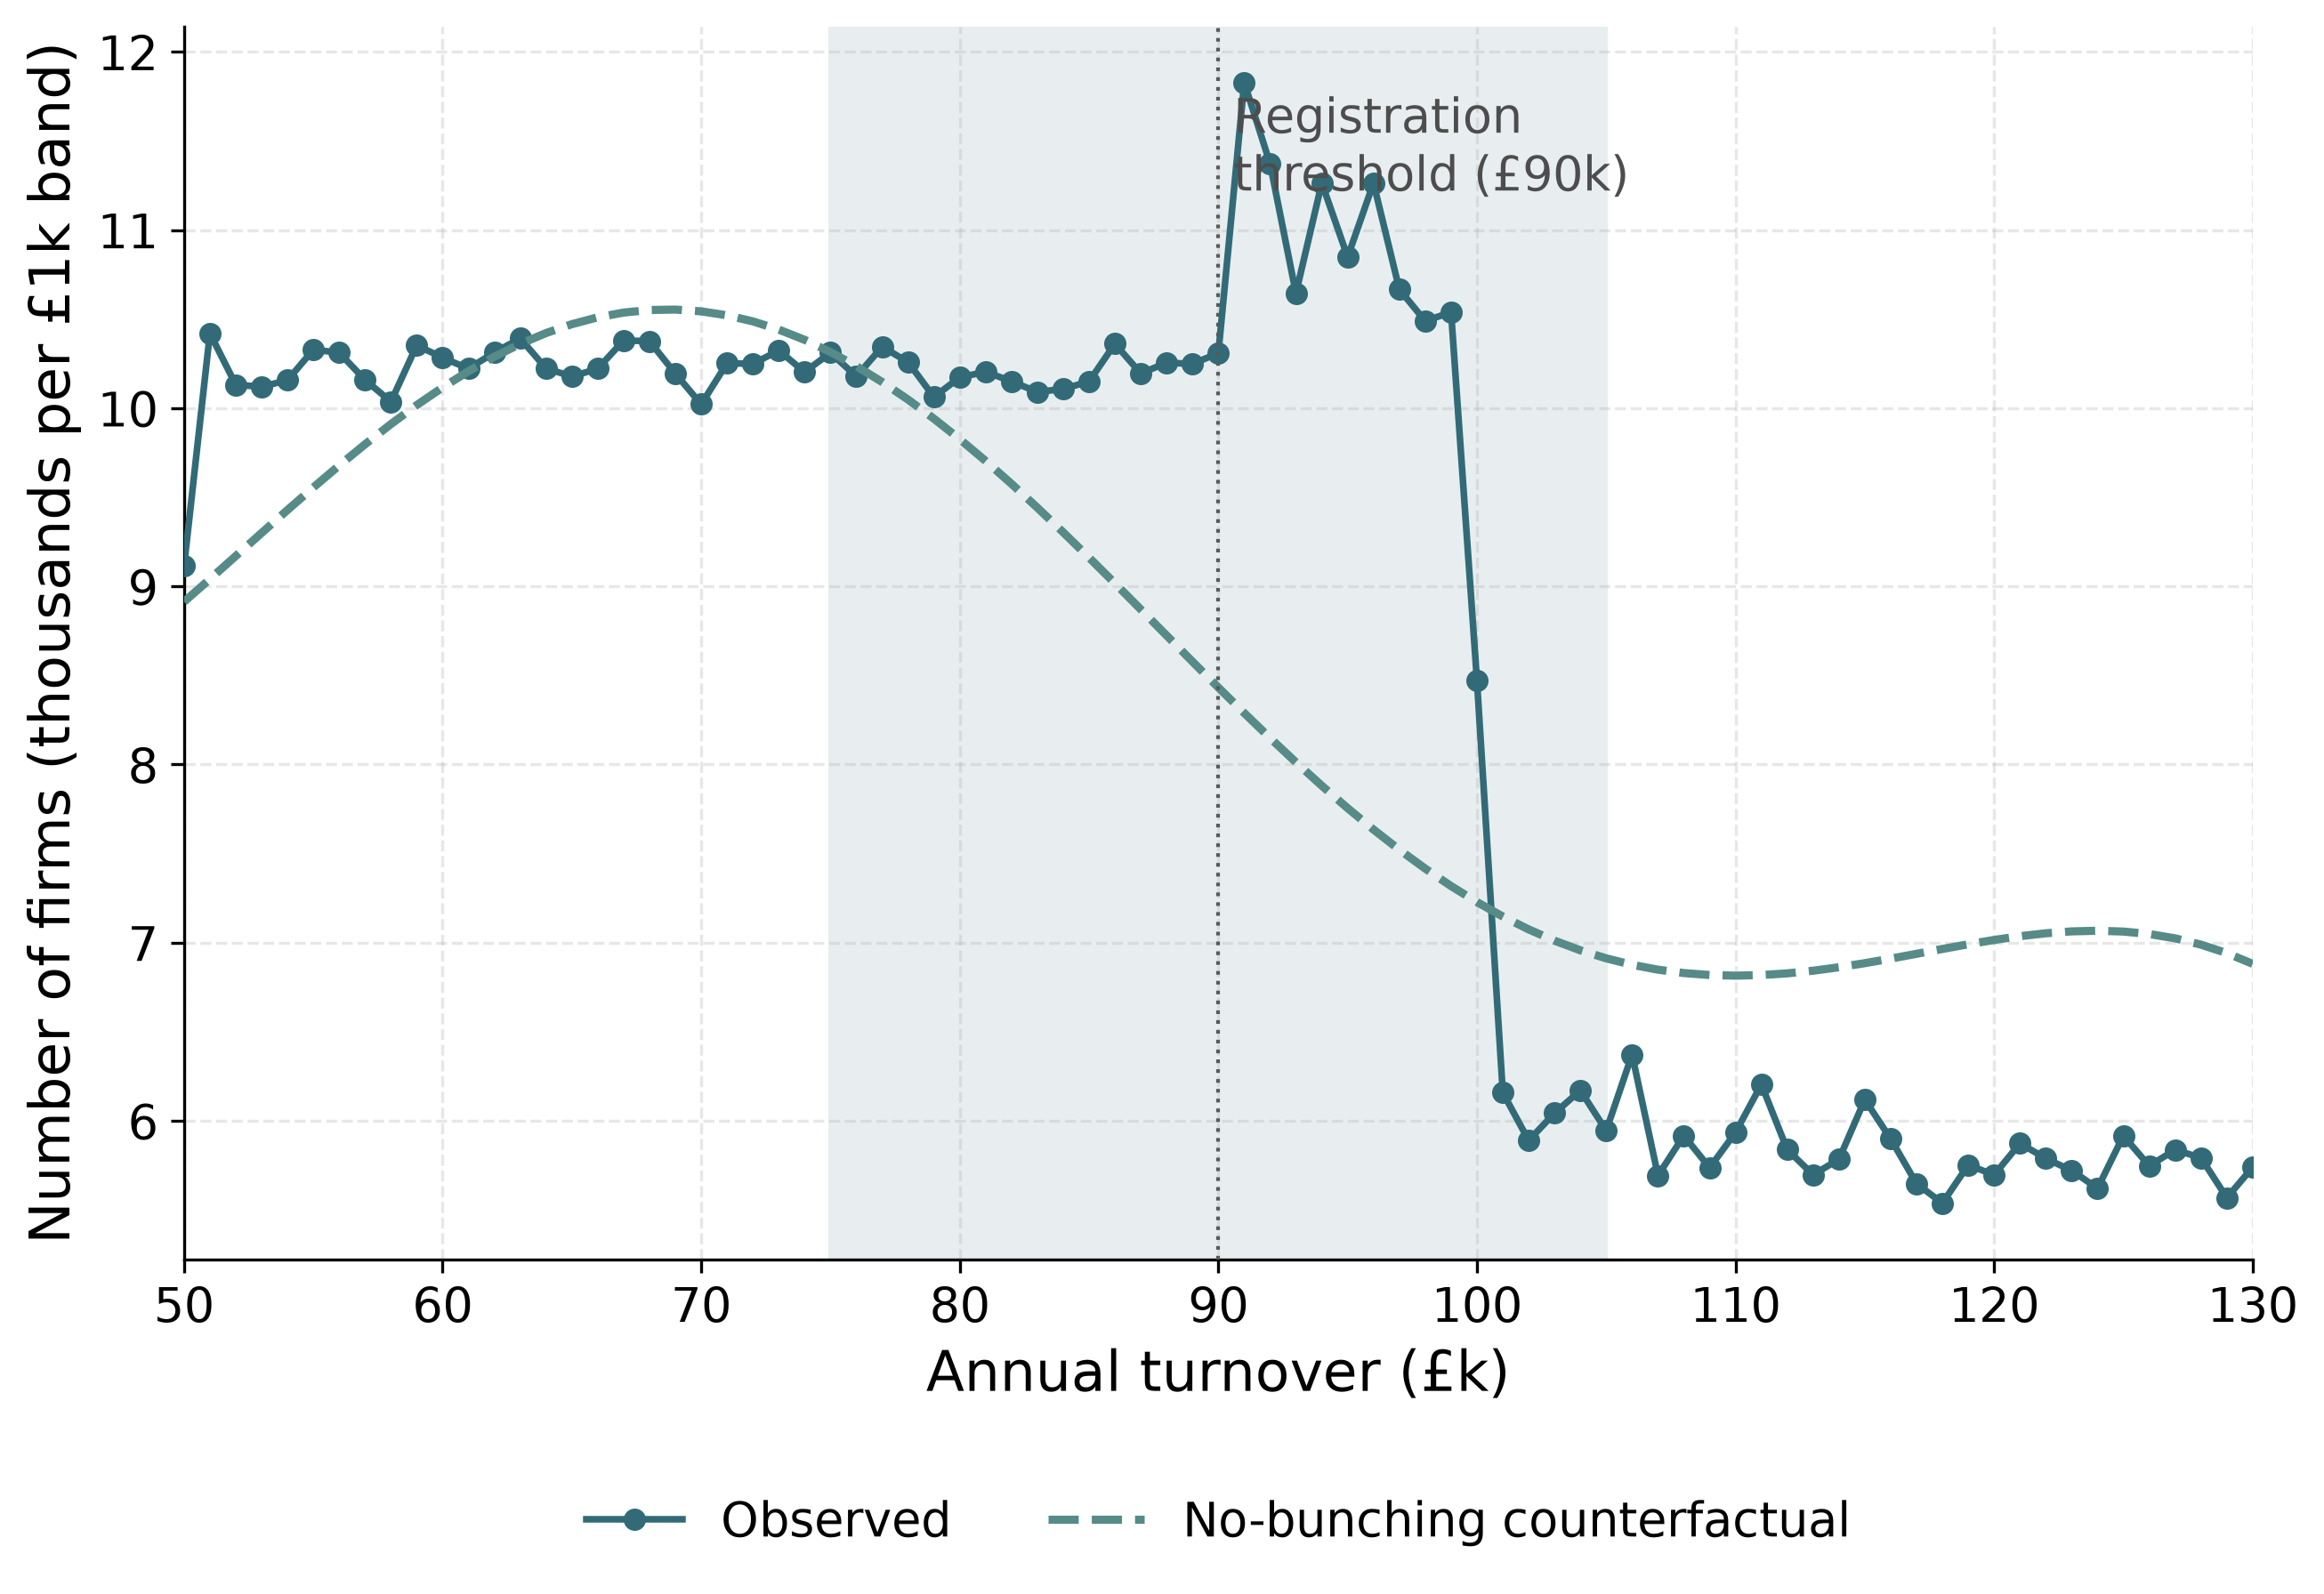
\includegraphics[width=0.48\textwidth]{figures/bunching_analysis_90k.png}
}
\caption{Observed synthetic firm density and polynomial no-bunching
counterfactual at each vintage's registration threshold. Panel (a): the
2023--24 population reproduces the administratively observed bunching profile
because it is calibrated to the OBR \pounds1{,}000-band targets; the
estimator reads the target-inherited excess back as $E = 14{,}663$
($b = 0.109$). Panel (b): the 2024--25 population, which has no fine targets,
shows a very large spurious signal at \pounds90{,}000
($E \approx 196{,}000$ weighted firms) at the HMRC calibration-band edge.
Neither is behavioural: the generator has no firm location-choice, so all
sub-band structure is inherited from the targets and the weight optimiser.}
\label{fig:bunch85}
\end{figure}

\subsection{Placebo test}
\label{ssec:bunch-placebo}

The placebo diagnoses where any threshold-adjacent structure comes from by
manipulating the calibration targets directly. HMRC publishes turnover counts
only in coarse bands across the threshold: in 2023--24, $678{,}350$ firms at
or below \pounds85{,}000 (about $7{,}981$ per \pounds1{,}000) against
$305{,}320$ between \pounds85{,}000 and \pounds150{,}000 (about $4{,}697$ per
\pounds1{,}000), so a band-average step is present in the target before any
firm is generated. In Placebo~A I reweight the synthetic firms so the
per-\pounds1{,}000 density follows a single smooth trend across the threshold,
holding total mass fixed. In Placebo~B I regenerate the entire population and
re-calibrate from scratch with \emph{no} fine structure in the targets at
all: the OBR near-threshold bins are removed and the two HMRC band counts
straddling the threshold are replaced by a split implied by one common
density. The results track the targets exactly. The control---calibrated to
the OBR profile---returns $E = 14{,}663$ ($b = 0.109$); Placebo~A returns
$E = 323$ ($b = -0.014$); Placebo~B returns $E = 0$ ($b = -0.274$). Deleting
the fine targets deletes the ``bunching''; and where a coarse step is present
in the targets---as at the 2024--25 vintage's \pounds90{,}000 band edge---the
estimator faithfully reads it as (spurious) mass. Inserting or removing
structure in the targets inserts or removes ``bunching'' in the estimates.

\subsection{Power (recovery) test}
\label{ssec:bunch-recovery}

A null result is only informative if the estimator could have detected a
signal. I therefore inject a Kleven--Waseem-consistent behavioural response of
known magnitude into the step-free (Placebo~A) population: firms relocate to
just below the threshold from a donor region extending to a true marginal
buncher at \pounds112{,}000---beyond the estimator's exclusion window, as with
genuine bunching---with relocation probability declining linearly in distance
from the threshold. Scored by the headline estimator with no reference to the
known null, injected excess masses of $2{,}000$, $5{,}000$ and $8{,}000$
weighted firms are recovered at $55\%$, $75\%$ and $82\%$ respectively, with
the estimated marginal-buncher location attenuated toward the threshold
(\pounds87{,}700--\pounds95{,}100 against the true \pounds112{,}000). The
attenuation has a measured mechanical source: part of the missing-mass region
lies outside the exclusion window, where it pulls the fitted counterfactual
down. The estimator therefore \emph{under}-states a true response, more
severely for small ones, and does not over-state one---so the target-inherited
$E=14{,}663$ at \pounds85{,}000 is, if anything, an attenuated reading of the
targeted profile, while the \pounds90{,}000 artifact is far too large for
attenuation to explain away.\footnote{An earlier
version of this exercise relocated mass entirely within the exclusion window,
which the counterfactual fit cannot see by construction; its reported
``$\sim$90\% recovery'' measured deposit bookkeeping, not estimator power. The
redesigned test is in \texttt{analysis/recovery\_bunching.py}.}

\subsection{Comparison with the literature}
\label{ssec:bunch-lit}

The behavioural fact in the literature is administrative. \citet{liuetal2021}
(hereafter LLAT) document genuine bunching at the UK VAT registration notch in
HMRC micro-data over 2004--05 to 2014--15, during which the threshold rose
from \pounds58{,}000 to \pounds81{,}000, with an excess-bunching ratio of
$b = 1.361$ (SE $0.202$) around the year-specific threshold and a manipulation
window of $-\pounds14{,}000$ to $+\pounds24{,}000$. My data's
$b_{\mathrm{LLAT}} = 2.86$ is not a second estimate of their parameter: it is
the OBR target profile read back through their normalisation, on a
deeper-bunching era.\footnote{The earlier draft's
$b_{\mathrm{LLAT}} = 0.94$, read against LLAT's $1.361$, illustrated how a
band-inherited artifact can land in the publishable range of the literature;
that artifact's disappearance under the liability correction, and its
replacement by an explicit published-data target, are reported above.} What does
carry across is institutional context: LLAT report that almost half (roughly
$43\%$) of eligible below-threshold firms register voluntarily, which dampens
observed bunching relative to a pure notch and which motivates the
voluntary-retention sensitivity of Section~\ref{sec:static}. For wider
order-of-magnitude context, \citet{obr2023vat} count firms holding turnover
below the frozen threshold over a \emph{wide} band (rising from $23{,}000$ in
2017--18 to about $44{,}000$ in 2025--26, with foregone turnover of
\pounds110m rising to \pounds350m); this is a different object from a
near-threshold spike and is cited only as context.

\subsection{Reduced-form evidence and the dominated region}

These results sharpen, rather than weaken, the case for grounding the policy
analysis in structure. The reduced-form density around the threshold cannot
price reforms---it has no single point of excess mass to forward-map onto a
change in the \emph{shape} of the schedule---and on band-calibrated synthetic
data it cannot be read behaviourally at all, in either direction. What the
structure of Section~\ref{sec:model} \emph{does} deliver exactly, for every
reform considered, is the notch's dominated region and how each schedule
change alters it. It is precisely because the reduced-form bunching is
non-identifying here that the exact dominated region carries the distortion
characterisation. The behavioural layer that re-prices each firm's turnover
under counterfactual schedules---conditional on an assumed turnover
elasticity---is developed in Section~\ref{sec:behavioural}.
